% SOURCE: Trigonometry With Tau as Circle Constant
% LINK: http://taufortrig.org/source_code_trigonometry_with_tau.html

\usepackage{tkz-euclide}
\usepackage{etoolbox}
\usepackage{MnSymbol}
% \usetkzobj{all}
\usetikzlibrary{angles,patterns,calc}
\usepackage[most]{tcolorbox}
\usepackage{pgfplots}
\pgfplotsset{compat=1.7}

~~~~

\definecolor{linecolor}{HTML}{0074C8}
\providecommand{\ival}[2]{\lbrack #1,#2 \rbrack}

\begin{tikzpicture}[scale=1.2,every node/.style={font=\small}]
\begin{scope}[dashed,line width=1pt,x=6cm/360]
\draw[black!60,solid,line width=0.3pt,-latex] (-110,0) -- (290,0) node[right] {$x$};
\draw[black!60,solid,line width=0.3pt,-latex] (0,-1.5) -- (0,1.5) node[above] {$y$};
\pgfplothandlerlineto
\pgfplotfunction{\x}{-90,-85,...,270}{\pgfpointxy{\x}{cos(\x)}}
\pgfusepath{stroke}
\node[black,below right] at (0,0) {$0$};
\foreach \pos in {-90,90,180,270}
\draw[black!60,line width=0.3pt,solid,shift={(\pos,0)}] (0pt,3pt) -- (0pt,-3pt);
\foreach \pos in {-1,1}
\draw[black!60,line width=0.3pt,solid,shift={(0,\pos)}] (3pt,0pt) -- (-3pt,0pt)
    node[black,left] {$\pos$};
\node[black,below] at (90,-0.1) {$\tfrac{\tau}{4}$};
\node[black,below] at (180,-0.1) {$\tfrac{\tau}{2}$};
\node[black,below] at (-90,-0.1) {$-\tfrac{\tau}{4}$};
\node[black,below] at (270,-0.1) {$\tfrac{3\tau}{4}$};
\node[black,above] at (90,1) {$y=\cos\;x$};
\end{scope}
\begin{scope}[color=linecolor,line width=1.5pt,x=6cm/360]
\pgfplothandlerlineto
\pgfplotfunction{\x}{0,5,...,180}{\pgfpointxy{\x}{cos(\x)}}
\pgfusepath{stroke}
\fill (0,1) circle (2pt);
\fill (180,-1) circle (2pt);
\end{scope}
\end{tikzpicture}\vspace{-6mm}